\documentclass[11pt,class=report,crop=false]{standalone}
\usepackage[screen]{../python}

\begin{document}


%====================================================================
\chapitre{Si ... alors ...}
%====================================================================

\objectifs{L'ordinateur peut réagir en fonction d'une situation. 
Si une condition est remplie il agit d'une certaine façon, 
sinon il fait autre chose.}


\insertvideo{tjZQ64VjvaU}{Si ... alors ... - partie 1}

\insertvideo{UlSmDST7zfk}{Si ... alors ... - partie 2 - entrée au clavier}

\insertvideo{ll5RENiJZwU}{Hasard - Module random}

\insertvideo{WNJRn4LbxXs}{Si ... alors ... - partie 3 - booléens}


%%%%%%%%%%%%%%%%%%%%%%%%%%%%%%%%%%%%%%%%%%%%%%%%%%%%%%%%%%%%%%%%
%%%%%%%%%%%%%%%%%%%%%%%%%%%%%%%%%%%%%%%%%%%%%%%%%%%%%%%%%%%%%%%%

\begin{cours}[Si ... alors ...]

Voici comment utiliser le test \og{}\ci{if}\fg{} avec \Python{} :
\index{si/alors}
\index{if@\ci{if}}

\mybox{
\myfigure{0.7}{
  \tikzinput{fig-sialors-cours-1}
} }

Voici un exemple, qui avertit un conducteur si une variable \ci{vitesse} est trop grande.
\begin{center}
\begin{minipage}{0.5\textwidth}
\begin{lstlisting}
if vitesse > 110:
    print("Attention, tu roules trop vite.")
\end{lstlisting}
\end{minipage} 
\end{center} 

On peut aussi exécuter des instructions si la condition n'est pas remplie à l'aide du mot \og{}\ci{else}\fg{}.
\index{sinon}
\index{else@\ci{else}}

\mybox{
\myfigure{0.7}{
  \tikzinput{fig-sialors-cours-2}
} }

Encore une fois c'est l'indentation qui délimite les différents blocs d'instructions.
Voici un exemple qui affiche le signe d'un nombre \ci{x}.
\begin{center}
\begin{minipage}{0.5\textwidth}
\begin{lstlisting}
if x >= 0:
    print("Le nombre est positif.")
else:
    print("Le nombre est négatif.")
\end{lstlisting}
\end{minipage} 
\end{center} 


\end{cours}


%%%%%%%%%%%%%%%%%%%%%%%%%%%%%%%%%%%%%%%%%%%%%%%%%%%%%%%%%%%%%%%%
%%%%%%%%%%%%%%%%%%%%%%%%%%%%%%%%%%%%%%%%%%%%%%%%%%%%%%%%%%%%%%%%

\begin{cours}[Entrée au clavier]

\index{entree@entrée}

Pour pouvoir interagir avec l'utilisateur, tu peux lui demander de saisir un texte au clavier.
Voici un petit programme qui demande le prénom et l'âge de l'utilisateur et affiche un message du style \og{}Bonjour Kevin\fg{} puis \og{}Tu es mineur/majeur !\fg{} selon l'âge.

\begin{center}
\begin{minipage}{0.5\textwidth}
\begin{lstlisting}
prenom = input("Comment t'appelles-tu ? ")
print("Bonjour",prenom)

age_chaine = input("Quel âge as-tu ? ")
age = int(age_chaine)

if age >= 18:
    print("Tu es majeur !")
else:
    print("Tu es mineur !")
\end{lstlisting}
\end{minipage} 
\end{center} 

\emph{Explications.}
\begin{itemize}
  \item La commande \ci{input()}\index{input@\ci{input}}
  met en pause l'exécution du programme et attend de l'utilisateur un texte (qu'il termine en appuyant sur la touche \og{}Entrée\fg{}).
  
  \item Cette commande renvoie une chaîne de caractères.
  
  \item \index{int@\ci{int}} Si on veut un entier, il faut convertir la chaîne. Par exemple, ici \ci{age_chaine} peut valoir
  \ci{"17"} (ce n'est pas un nombre mais une suite de caractères), alors que \ci{int(age_chaine)} vaut maintenant l'entier \ci{17}. 
  
  \item \index{str@\ci{str}} L'opération inverse est aussi possible, \ci{str()} convertit un nombre en une chaîne. Par exemple \ci{str(17)} renvoie la chaîne \ci{"17"} ; si \ci{age = 17}, alors \ci{str(age)} renvoie également \ci{"17"}.
\end{itemize}

\end{cours}

%%%%%%%%%%%%%%%%%%%%%%%%%%%%%%%%%%%%%%%%%%%%%%%%%%%%%%%%%%%%%%%%
%%%%%%%%%%%%%%%%%%%%%%%%%%%%%%%%%%%%%%%%%%%%%%%%%%%%%%%%%%%%%%%%

\begin{cours}[Le module \og{}random\fg{}]

\index{hasard}
\index{random@\ci{random}}
\index{module!random@\ci{random}}

Le module \ci{random} génère des nombres comme s'ils étaient tirés au hasard.
\begin{itemize}
  \item Voici la commande à placer au début du programme pour appeler ce module :\\
  \centerline{\ci{from random import *}}
  
  \item La commande \ci{randint(a,b)}\index{randint@\ci{randint}} renvoie un entier au hasard compris entre $a$ et $b$.
  
  Par exemple après l'instruction \ci{n = randint(1,6)}, $n$ est un entier tiré au hasard avec $1 \le n \le 6$.
  Si on recommence l'instruction \ci{n = randint(1,6)}, $n$ prend une nouvelle valeur. C'est comme si on effectuait le lancer d'un dé à $6$ faces.
  
  \item La commande \ci{random()}, sans argument, renvoie un nombre flottant (c'est-à-dire un nombre à virgule) compris  entre $0$ et $1$.  
  Par exemple, après l'instruction \ci{x = random()}, alors $x$ est un nombre flottant avec $0 \le x < 1$.
\end{itemize}


\end{cours}


%%%%%%%%%%%%%%%%%%%%%%%%%%%%%%%%%%%%%%%%%%%%%%%%%%%%%%%%%%%%%%%%
% Activité 1
%%%%%%%%%%%%%%%%%%%%%%%%%%%%%%%%%%%%%%%%%%%%%%%%%%%%%%%%%%%%%%%%

\begin{activite}[Quiz multiplications]

\objectifs{Objectifs : programmer un petit test sur les tables de multiplication.}

\begin{itemize}
  \item Définis une variable $a$, à laquelle tu affectes une valeur au hasard entre $1$ et $12$.
  
  \item Même chose pour une variable $b$.
  
  
  \item Affiche à l'écran la question : \og{}Combien vaut le produit $a \times b$ ?\fg{}
  (Remplace $a$ et $b$ par leur valeur !)
  
  \item Récupère la réponse de l'utilisateur et transforme-la en un entier.
  
  \item Si la réponse est correcte affiche \og{}Bravo !\fg{}, sinon affiche \og{}Perdu ! La bonne réponse était\ldots\fg{}.
\end{itemize}


\mybox{
\textbf{Test d'égalité.} Pour tester si deux nombres $x$ et $y$ sont égaux, l'instruction est :\\
\centerline{\ci{if x == y:}}
Le test d'égalité s'écrit bien avec le double signe égal \og{}\ci{==}\fg{}.
Par exemple \og{}\ci{x == 3}\fg{} renvoie \og{}vrai\fg{} si $x$ vaut $3$ et \og{}faux\fg{} sinon.

Attention ! La commande \og{}\ci{x = 3}\fg{} n'a rien à voir, cette instruction stocke $3$ dans la variable $x$.
}

\end{activite}


%%%%%%%%%%%%%%%%%%%%%%%%%%%%%%%%%%%%%%%%%%%%%%%%%%%%%%%%%%%%%%%%
% Activité 2
%%%%%%%%%%%%%%%%%%%%%%%%%%%%%%%%%%%%%%%%%%%%%%%%%%%%%%%%%%%%%%%%

\begin{activite}[Les mots de la tortue]

\objectifs{Objectifs : piloter la tortue par un mot, chaque caractère correspondant à une instruction.}

Tu donnes un mot à la tortue \Python, par exemple \mot{AgAdaagAdaA}, dans lequel chaque caractère (lus de gauche à droite) correspond à une instruction que la tortue doit exécuter.

\begin{itemize}
  \item \mot{A} : avance de $100$ en traçant,
  \item \mot{a} : avance de $100$ sans tracer,  
  \item \mot{g} : tourne à gauche de $90$ degrés,
  \item \mot{d} : tourne à droite de $90$ degrés.
\end{itemize}

\emph{Exemple.}
Voici le dessin que doit tracer la tortue lorsque \ci{mot} vaut \ci{"AagAgAdAgAAgaAA"}. 

\begin{center}
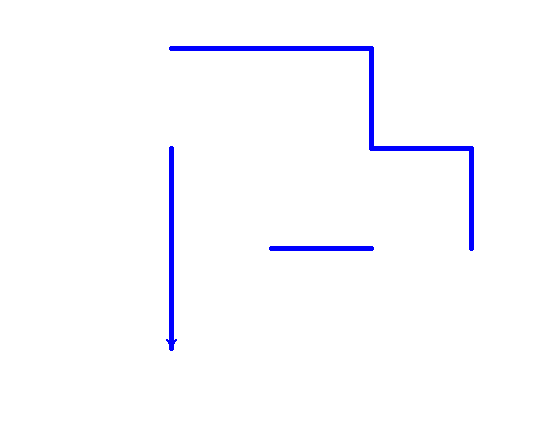
\includegraphics[scale=\myscale,scale=0.4]{ecran-sialors-2}
\end{center}

\emph{Indications.}
Voici comment parcourir les lettres d'un mot et tester si une lettre est le caractère \mot{A} :
\begin{center}
\begin{minipage}{0.5\textwidth}
\begin{lstlisting}
for c in mot:
    if c == "A":
        instructions...
\end{lstlisting}
\end{minipage} 
\end{center} 

   
\end{activite}



%%%%%%%%%%%%%%%%%%%%%%%%%%%%%%%%%%%%%%%%%%%%%%%%%%%%%%%%%%%%%%%%
%%%%%%%%%%%%%%%%%%%%%%%%%%%%%%%%%%%%%%%%%%%%%%%%%%%%%%%%%%%%%%%%

\begin{cours}[Booléens]
\sauteligne
\begin{itemize}
  \item Un \defi{booléen}\index{booleen@booléen} est une donnée qui vaut soit la valeur \og{}vrai\fg{}, soit la valeur \og{}faux\fg{}. En \Python{} les valeurs sont \ci{True}\index{true@\ci{True}} et \ci{False}\index{false@\ci{False}} (avec une majuscule).
  
  \item On obtient un booléen par exemple comme résultat de la comparaison de deux nombres.
  Par exemple \ci{7 < 4} vaut \ci{False} (car $7$ n'est pas plus petit que $4$). 
  Vérifie que \ci{print(7 < 4)} affiche \ci{False}.
  
  Voici les principales comparaisons :
  \begin{itemize}
    \item \textbf{Test d'égalité :}\quad \ci{a == b}\index{\ci{==}}
    	\item \textbf{Test inférieur strict :}\quad \ci{a < b}
    	\item \textbf{Test inférieur large :}\quad \ci{a <= b}\index{\ci{<=}}
    	\item \textbf{Test supérieur :}\quad \ci{a > b} \quad ou \quad \ci{a >= b}\index{\ci{>=}}
    	\item \textbf{Test non égalité :}\quad \ci{a != b}\index{\ci{"!}\ci{=}}
  \end{itemize}
   
   Par exemple \ci{6*7 == 42} vaut \ci{True}.
   

   
   
   \item ~\index{affectation}\index{=@\ci{=}}
   \mybox{
   \textbf{ATTENTION !}   
   L'erreur classique est de confondre \og{}\ci{a = b}\fg{} et \og{}\ci{a == b}\fg{}.
   \begin{itemize}
     \item \textbf{Affectation.} \ci{a = b}
     met le contenu de la variable \ci{b} dans la variable \ci{a}.
     \item \textbf{Test d'égalité.} \ci{a == b} teste si les contenus de \ci{a} et de \ci{b} sont égaux et vaut \ci{True} ou \ci{False}.
   \end{itemize}
   }
   
  \item On peut comparer autre chose que des nombres. Par exemple 
  \og{}\ci{car == "A"}\fg{} teste si la variable \ci{car} vaut \ci{"A"} ; \og{}\ci{il_pleut == True}\fg{} teste si la variable \ci{il_pleut} est vraie\ldots
  
  \item Les booléens sont utiles dans le test \og{}si \ldots{} alors \ldots\fg{} et dans les boucles \og{}tant que \ldots{} alors \ldots\fg{}.
  
  \item \textbf{Opérations entre les booléens.}
  \index{operation logique@opération logique}
  Si $P$ et $Q$ sont deux booléens, on peut définir de nouveaux booléens.
  \begin{itemize}
    \item \textbf{Et logique.}\index{et}\quad \og{}\ci{P and Q}\fg{}\index{and@\ci{and}} est vrai si et seulement si $P$ et $Q$ sont vrais.
    	\item \textbf{Ou logique.}\index{ou}\quad \og{}\ci{P or Q}\fg{}\index{or@\ci{or}} est vrai si et seulement si $P$ ou $Q$ est vrai.
    	\item \textbf{Négation.}\index{non}\quad \og{}\ci{not P}\fg{}\index{not@\ci{not}} est vrai si et seulement si $P$ est faux.
  \end{itemize}  
  
  Par exemple \og{}\ci{(2+2 == 2*2) and (5 < 3)}\fg{} renvoie \ci{False}, car
  même si on a bien $2+2 = 2 \times 2$, l'autre condition n'est pas remplie car $5 < 3$ est faux.
  
  
  
\end{itemize}
\end{cours}




%%%%%%%%%%%%%%%%%%%%%%%%%%%%%%%%%%%%%%%%%%%%%%%%%%%%%%%%%%%%%%%%
% Activité 3
%%%%%%%%%%%%%%%%%%%%%%%%%%%%%%%%%%%%%%%%%%%%%%%%%%%%%%%%%%%%%%%%

\begin{activite}[Chiffres d'un nombre]

\objectifs{Objectifs : trouver des nombres dont les chiffres vérifient certaines propriétés.}
\index{ecriture@écriture!decimale@décimale}

\begin{enumerate}
  \item Le programme suivant affiche tous les entiers de $0$ à $99$. Comprends ce programme. Que représentent les variables $u$ et $d$ ?
  
\begin{center}
\begin{minipage}{0.5\textwidth}
\begin{lstlisting}
for d in range(10):
    for u in range(10):
        n  = 10*d + u
        print(n)
\end{lstlisting}
\end{minipage} 
\end{center} 
  
  \item Trouve tous les entiers compris entre $0$ et $999$ qui vérifient toutes les propriétés suivantes :
  \begin{itemize}
    \item l'entier se termine par $3$,
    
    \item la somme des chiffres est supérieure ou égale à $15$,
    
    \item le chiffre des dizaines est pair.
  \end{itemize}
   
  
  \item Modifie ton programme précédent pour compter et afficher le nombre d'entiers vérifiant les propriétés.
  
\end{enumerate}

\end{activite}



%%%%%%%%%%%%%%%%%%%%%%%%%%%%%%%%%%%%%%%%%%%%%%%%%%%%%%%%%%%%%%%%
% Activité 4
%%%%%%%%%%%%%%%%%%%%%%%%%%%%%%%%%%%%%%%%%%%%%%%%%%%%%%%%%%%%%%%%

\begin{activite}[Triangles]

\objectifs{Objectifs : déterminer les propriétés d'un triangle à partir des trois longueurs des côtés.}
\index{triangle}

On se donne trois longueurs $a$, $b$ et $c$. Tu vas déterminer les propriétés du triangle dont les longueurs seraient $a$, $b$, $c$.

\myfigure{1}{
\tikzinput{fig-sialors-1}
}  


Définis trois variables $a$, $b$ et $c$ avec des valeurs entières et $a \le b \le c$
(ou bien demande à l'utilisateur trois valeurs).

\begin{enumerate}
  \item \textbf{Ordre.} Demande à \Python{} de tester si les longueurs vérifient bien $a \le b \le c$. Affiche une phrase pour la réponse.
  
  \item \textbf{Existence.} Il existe un triangle correspondant à ces longueurs si et seulement si :
  $$a + b \ge c.$$
  Demande à \Python{} de tester si c'est le cas et affiche la réponse.
  
  
  \item  \textbf{Triangle rectangle.} Demande à \Python{} de tester si le triangle est un triangle rectangle. (Pense au théorème de Pythagore.)
  
   \item  \textbf{Triangle équilatéral.} Teste si le triangle est équilatéral. 
   
   \item  \textbf{Triangle isocèle.} Teste si le triangle est isocèle.   
   
   \item  \textbf{Angles aigus.} Teste si tous les angles sont aigus (c'est-à-dire inférieurs ou égaux à $90$ degrés).
   
    \emph{Indications.} 
    \begin{itemize}
      \item La loi des cosinus permet de calculer un angle en fonction des longueurs :
      
 \myfigure{1}{
\tikzinput{fig-sialors-3}
}   
   
   $$\cos \alpha = \frac{-a^2+b^2+c^2}{2bc},
   \qquad
   \cos \beta = \frac{a^2-b^2+c^2}{2ac},
   \qquad
   \cos \gamma = \frac{a^2+b^2-c^2}{2ab}.$$   

   \smallskip
   
    \item Pour tester si l'angle $\alpha$ est aigu il suffit de vérifier $\cos \alpha \ge 0$ (au final on ne calcule jamais $\alpha$, mais juste $\cos \alpha$).
   
   \end{itemize} 
   
\end{enumerate}   
     
    \objectifs{Trouve des exemples de longueurs $a,b,c$ pour illustrer les différentes propriétés.}
    
\end{activite}


%%%%%%%%%%%%%%%%%%%%%%%%%%%%%%%%%%%%%%%%%%%%%%%%%%%%%%%%%%%%%%%%
% Activité 5
%%%%%%%%%%%%%%%%%%%%%%%%%%%%%%%%%%%%%%%%%%%%%%%%%%%%%%%%%%%%%%%%

\begin{activite}[Le nombre mystère]

\objectifs{Objectifs : coder le jeu incontournable lorsque l'on apprend à programmer. L'ordinateur choisit un nombre au hasard. L'utilisateur doit deviner ce nombre en suivant des indications \og{}plus grand\fg{} ou \og{}plus petit\fg{} données par l'ordinateur. Comme ce jeu est vite lassant, on introduit des variantes où l'ordinateur a le droit de mentir ou de tricher !}


\begin{enumerate}
  \item \textbf{Le jeu classique.}
  \begin{itemize}
    \item L'ordinateur choisit au hasard un nombre mystère entre $0$ et $99$.
    \item Le joueur propose une réponse.
    \item L'ordinateur répond 
    \og{}le nombre à trouver est plus grand\fg{} ou
     \og{}le nombre à trouver est plus petit\fg{} ou
      \og{}bravo, c'est le bon nombre !\fg{}. 
     \item Le joueur a sept tentatives pour trouver la bonne réponse.
  \end{itemize}
  
  Programme ce jeu !
  
  \emph{Indications.} Pour quitter une boucle \ci{for} avant la dernière proposition, tu peux utiliser la commande \ci{break}. Utilise ceci lorsque le joueur trouve la bonne réponse.

  
  \item \textbf{L'ordinateur ment.}
  
  Pour compliquer le jeu, l'ordinateur a le droit de mentir de temps en temps.
  Par exemple environ une fois sur quatre l'ordinateur donne la mauvaise indication \og{}plus grand\fg{}
  ou \og{}plus petit\fg{}.
  
  \emph{Indications.} Pour décider quand l'ordinateur ment, à chaque tour tire un nombre au hasard entre $1$ et $4$, si c'est $4$ l'ordinateur ment !
  
  
  
  
  \item \textbf{L'ordinateur triche.}
  
  Maintenant l'ordinateur triche (mais il ne ment plus) ! À chaque tour l'ordinateur change un peu le nombre mystère à trouver.
  
    \emph{Indications.} À chaque tour, tire un nombre au hasard, entre $-3$ et $+3$ par exemple, et ajoute-le au nombre mystère. (Attention à ne pas dépasser les bornes $0$ et $99$.)
  
\end{enumerate}   
     
\end{activite}

\end{document}
